\subsection{Correct Lifting of a Quad-Copter Stabilization Algorithm}

We evaluated InteGreat\ by recovering equations for continuous orientation estimation from an open-source, MCU-based quad-copter autopilot controller.
The firmware we studied implemented Madgwick's Gradient Descent Orientation Filter~\cite{madgwick}.
The orientation estimator takes in sensor inputs from the IMU consisting of an accelerometer, gyroscope, and magnetometer.
Orientation Estimators for strapdown INS (Inertial Navigation Systems) \emph{continuously} fuse sensor data with previous estimations and obtain new attitude across the time domain.
Because of this, difference in implementations that are subtle on the surface lead to large accumulative error across small time periods.

We ran four experiments using different versions of Madgwick's algorithm to showcase InteGreat's ability in detecting bugs and algorithm variants in firmware.
These experiments are depicted in Fig.~\ref{fig:madg}, through a simulation of the quad-copter spinning in three dimensions.
These simulations were performed using Matlab's ``rpy\_9axis'' sensor data.

\begin{figure*}
    \centering
    \begin{subfigure}[b]{0.327\textwidth}
        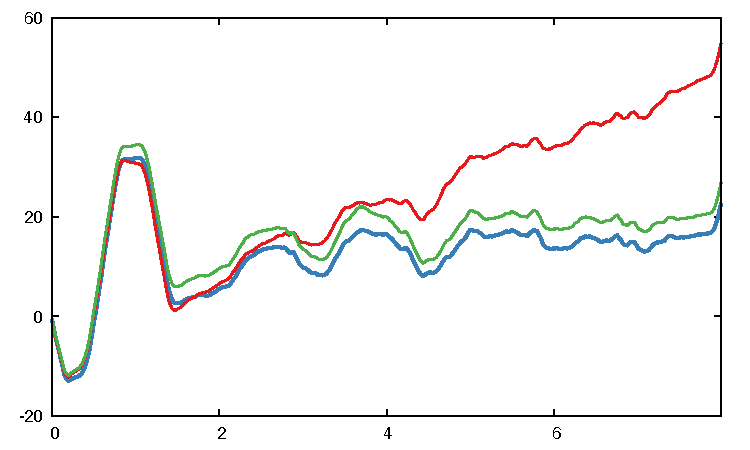
\includegraphics[width=\textwidth]{madg_data/pitch.pdf}
	    \caption{Pitch}
    \label{fig:pitch}
    \end{subfigure}
    \hfill
    \begin{subfigure}[b]{0.327\textwidth}
        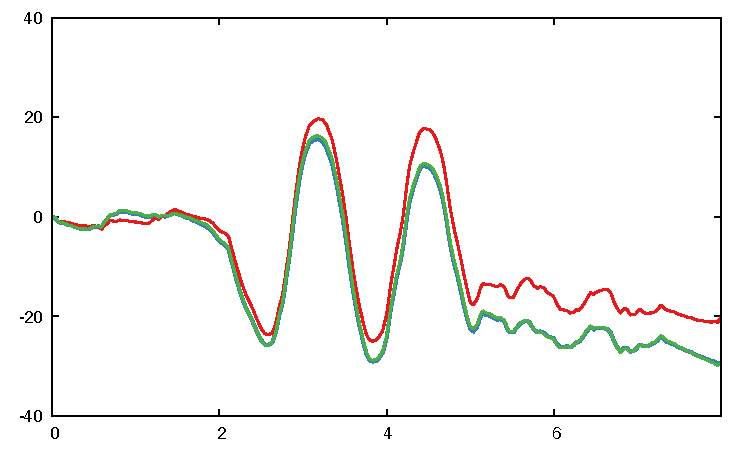
\includegraphics[width=\textwidth]{madg_data/yaw.pdf}
        \caption{Yaw}
        \label{fig:yaw}
    \end{subfigure}
    \hfill
    \begin{subfigure}[b]{0.327\textwidth}
        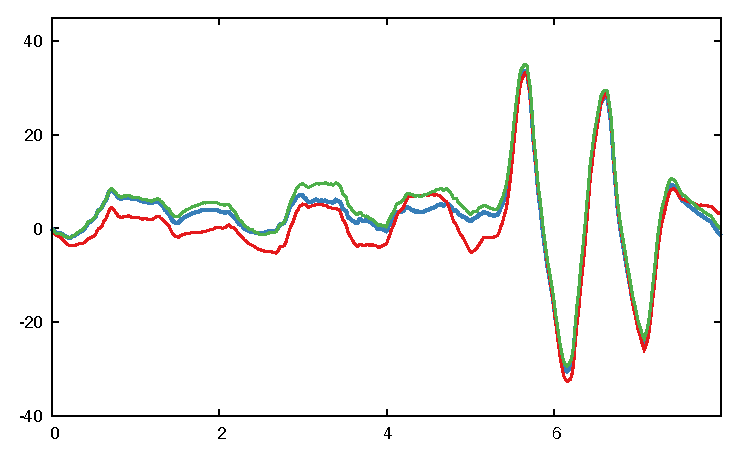
\includegraphics[width=\textwidth]{madg_data/roll.pdf}
        \caption{Roll}
        \label{fig:roll}
    \end{subfigure}
    \hfill
    \caption{Empirical results measuring the ability of InteGreat's recovered models of Orientation Estimation algorithms to identify bugs.}
    \label{fig:madg}
\end{figure*}

Note that only three lines are present in Fig.~\ref{fig:madg}.
The fourth line, the correct Matlab implementation, the blue line, is identical to lifted version of a corresponding correct C implementation.
This finding ensures InteGreat\ did not make mistakes while lifting, and was able to produce identically behaving Matlab code with respect to compiled C firmware code.
The equivalence between the two correct implementations gives us confidence in the methodology InteGreat\ introduces.

The figure depicts the same inputs to the IMU sensor of a device oscillating in pitch, yaw, then roll. \textbf{Green} is lifted by InteGreat\ from \emph{real world} firmware that contains a bug. \textbf{Blue} contains \emph{two} lines: the InteGreat\ lifted firmware recompiled to correct the gradient calculation, and \emph{a correct} Matlab implementation of Madgwick's algorithm. \textbf{Red}, however, is a compiled firmware using the \emph{faulty} C code included in Madgwick's published report. This version has accumulative error with respect to the earth's magnetic field.

Continuous equations lifted by InteGreat\ were identical to ground truth simulations in a controlled IMU sensor experiment rotating the quadcopter in 3 dimensions using 1,600 measurement points. This demonstrates our framework is able to lift correct continuous equations from discrete, machine code implementations and verify them using tools operating over the abstract domain.

\paragraph{Example of InteGreat Identifying Bugs}
\label{sec:quadcopter}

%Even the proposer of this algorithm published two variants, one C implementation in the appendix of his report and a Matlab implementation on his website after the Orientation Filter became increasingly popular for commodity drones ~\cite{}.

We next evaluate whether InteGreat\ is useful when attempting to identify bugs in firmware.
When comparing the Madgwick-provided Matlab implementation (blue) with the version recovered from the \emph{real world} firmware implementation (green), we discovered an error in the gradient of the solution surface which is calculated by multiplying the objective Function matrix and its Jacobian matrix: $\nabla F = \mathbf{J}^T(_{E}^{S}\hat{\mathbf{q}},^{E}\hat{\mathbf{b}}) \mathbf{F}(_{E}^{S}\hat{\mathbf{q}},^{E}\hat{\mathbf{b}}, ^{S}\hat{\mathbf{a}}, ^{S}\hat{\mathbf{m}})$.
Comparing the correct magnetic field components of the Objective Function with the InteGreat\ lifted version (using normalized magnetic field sensor values for simplicity):

\newcommand*{\Scale}[2][4]{\scalebox{#1}{$#2$}}%
$$
\mathbf{f}_b(_{E}^{S}\hat{\mathbf{q}},^{E}\hat{\mathbf{b}} ^{S}\hat{\mathbf{m}}) = 
\begin{bmatrix}
    2b_{x}(0.5-q_{3}^{2}-q_{4}^{2})+2b_{z}(q_{2}q_{4}-q_{1}q_{3})-m_{x}\\
    2b_{x}(q_{2}q_{3}-q_{1}q_{4})+2b_{z}(q_{1}q_{2}+q_{3}q_{4})-m_{y}\\
    2b_{x}(q_{1}q_{3}+q_{2}q_{4})+2b_{z}(0.5-q_{2}^{2}-q_{3}^{2})-m_{z}\\
\end{bmatrix}
$$

\[
\begin{aligned}
	F_4 &= ((0.5 + (- q_3 ^ 2 ) + (- q_4 ^ 2 ))  * b_x  + (q_2 * q_4  + (- q_1 * q_3 )) * b_z + (- m_x) \\
	F_5 &= (q_2 * q_3  + (- q_1 * q_4 )) * b_x + (q_3 * q_4 + q_1 * q_2) * b_z + (- m_y) \\
	F_6 &= (((0.5 + (- q_2 ^ 2)) + (- q_3 ^ 2))  * b_z  + (q_1 * q_3  + q_2 * q_4 ) * b_x + (- mz) \\
\end{aligned}
\]
\normalsize

It is clear that terms using the earth’s magnetic field ($^{E}\hat{\mathbf{b}}$) in the Objective Function have missing coefficients.\footnote{
	$b_{y}$ is not present as the earth’s magnetic field is be considered to have components in one horizontal axis and the vertical axis.}
The same errors occur in all magnetic field components of the Jacobian.
We compare only one row of the Jacobian here for simplicity:

\[
\begin{aligned}
    J_{4,1}&= (-q_3*b_z) \\
    J_{4,2}&= (q_4*b_z) \\
    J_{4,3}&= (q_3*(-2*b_x)+(-q_1*b_z)) \\
    J_{4,4}&= (q_4*(-2*b_x)+(q_2*b_z)) \\
\end{aligned}
\]
\[
\begin{aligned}
    \mathbf{J_4}(_{E}^{S}\hat{\mathbf{q}},^{E}\hat{\mathbf{b}}) &= \begin{bmatrix}
    -2b_zq_3, & 2b_zq_4, & -4b_xq_3-2b_zq_1,  & -4b_xq_4+2b_zq_2 \\
\end{bmatrix}\\
\end{aligned}
\]
\normalsize

%TODO: Is there something to be said about accumulated errors and how attacks can be made more stealthy?
After correcting all coefficients of the earth’s magnetic field ($^{E}\hat{\mathbf{b}}$) and recompiling the quad-copter firmware, the continuous equations lifted by InteGreat\ exactly matched Madgwick's Matlab implementation (blue).

We then compared the corrected equations (blue) with a \emph{third} firmware version, compiled to use Madgwick's published implementation, written in C, which is included in the original Madgwick paper (red).
We found that the published variant of the algorithm recursively feeds in previously calculated gyroscopic biases multiplied by a correction constant $\zeta$.
In contrast, existing implemented algorithms did \emph{not} perform gyroscopic bias removal and instead used dynamically calculated flux vectors of the Earth's frame in the equation's objective function.
This further confirmed InteGreat's ability to help researchers understand differences between implementations and published results.

% research question answer
By lifting compiled machine code to continuous equations using logical reasoning, it is possible to identify bugs in firmware implementations and check the validity of published results.
Validation can be performed by comparing representations which, after lifting, operate over the same domain, or by using a framework to check output equivalence, i.e. reachability, between algorithm versions.

% InteGreat's output was:
% $$
% \begin{aligned}
%     &w_{errz} = ((2 * q_1  * s_4) + (- 2 * q_2 * s_3)  + (2 * q_3 * s_2) + (- 2 * q_4 * s_1))\\
%     &w_{erry} = ((2 * q_1  * s_3)  + (2 * q_2 * s_4) + (- 2 * q_3 * s_1) + (- 2 * q_4 * s_2))\\
%     &w_{errx} = ((2 * q_1  * s_2)  + (- 2 * q_2 * s_1) + (- 2 * q_3 * s_4) + (2 * q_4 * s_3))\\
%     &w_{bz} = (w_{errz} * \zeta * \delta_t + w_{bz})\\
%     &w_{by} = (w_{erry} * \zeta * \delta_t + w_{bx})\\
%     &w_{bx} = (w_{errx} * \zeta * \delta_t + w_{by})\\
% \end{aligned}
% $$



% Taking in account the numerous different implementations of the Madgwick Orientation Filter, we consider a Madgwick Orientation Filter to be \emph{Correct} if the gradient calculation is the same as published in Madgwick's paper, and the gradient correctly updates the quaternion; \emph{Complete} if the Orientation estimation is within reasonable error range of the algorithm published by Madgwick.

% \begin{figure}
%     \centering
%     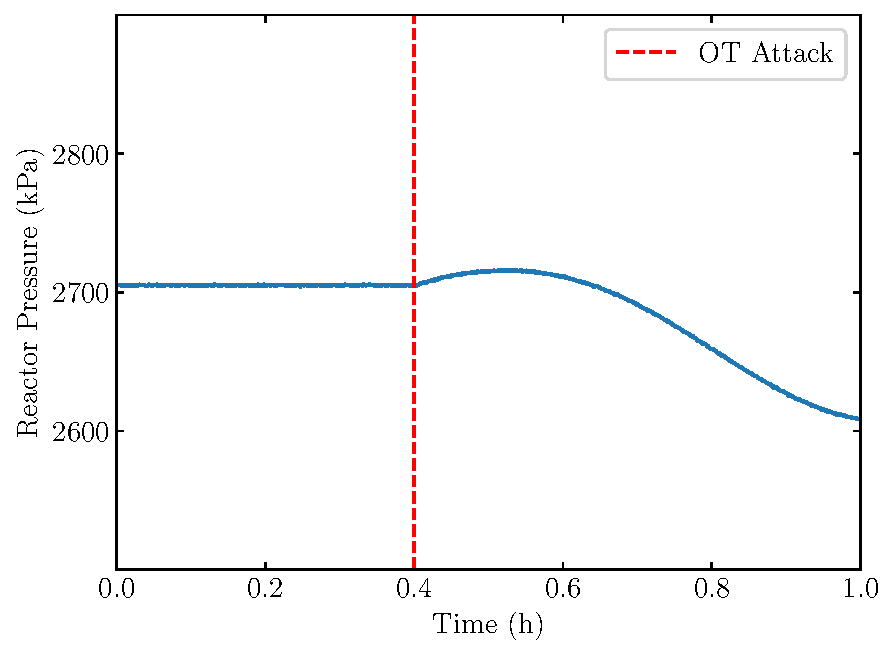
\includegraphics[width=0.4\textwidth]{plc_data/plot.pdf}
%     \caption{Simulated OT attack on the continuous equations \emph{lifted} from closed source, symbol-stripped PLC firmware.}
%     \label{fig:te_attack}
% \end{figure}




